\section{Combinators for Context-Free Path Querying}

In this section we demonstrate main features of combinators in the context of context-free path querying and integration with general-purpose programming languages.
To do it we first introduce a simple graph analysis problem and then show how to solve it by using parser combinators
In our wirk we use Merrkst.Graph combinators library.

\subsection{Problem Statement}
Suppose we have an RDF graph and whatn to analize hierarchical dependencies over different types of relations.
Our goal is for fhe given object to find all objects which lies on the same lavel of hierarchy!!!
!!!!!

\subsection{Graph Schema}
After graph loaded to the database first we should to do is to create typed schema: specify types of nodes oad edges.

\begin{lstlisting}
def sameGen2():Symbol[Entity,Entity,_] =
    syn(inE((_: Entity).label() == "skos__narrowerTransitive") ~ sameGen2 .? ~ (outE((_: Entity).label() == "skos__narrowerTransitive")))
\end{lstlisting}



\begin{lstlisting}

def reduceChoice[L, N, V](xs: List[Symbol[L, N, V]]): Symbol[L, N, V] = {
  xs match {
	case x :: Nil => x
	case x :: y :: xs =>
	  syn(xs.foldLeft(x | y)(_ | _))
  }
}
\end{lstlisting}


\begin{lstlisting}
def sameGen1[L, N, V]( brs: List[(Symbol[L, N, V], Symbol[L, N, V])]):Symbol[L,N,_] =
   reduceChoice(
	 brs.map {
	   case (lbr, rbr) => syn(lbr ~ (sameGen1(brs).?) ~ rbr)
	 }
   )
\end{lstlisting}

\begin{lstlisting}

def queryFromV1[L, N](startV: Symbol[L, N, _],
					 query: Symbol[L, N, _]) =
  syn(startV ~ query ~ uriV & {case _ ~ _ ~ (v:Entity) => v.getProperty[String]("uri")})
\end{lstlisting}

\begin{lstlisting}
def sameGen[L, N, V](
      brs: List[(Symbol[L, N, V], Symbol[L, N, V])]): Symbol[L, N, Int] =
    reduceChoice(
      brs.map {
        case (lbr, rbr) =>
          syn((lbr ~ (sameGen(brs).?) ~ rbr) & {
            case _~Nil~_ => 2
            case _~((x:Int)::Nil)~_ =>  x + 2
          })
      }
    )
\end{lstlisting}

\begin{lstlisting}
val uriV: Symbol[Entity, Entity, Entity] =
    syn(V((_: Entity).hasProperty("uri")) ^^)

  def queryFromV[L, N](startV: Symbol[L, N, _],
                               query: Symbol[L, N, _]) =
    syn(startV ~ query ~ uriV & {case _ ~ (len:Int) ~ (v:Entity) => (len, v.getProperty[String]("uri"))})
	\end{lstlisting}



\begin{lstlisting}
def runExample2(brs: List[String]) =
    runWithGraph({ graph: Input[Entity, Entity] =>
      val symbolBrs = brs
        .map(name =>
          (syn(inE((_: Entity).label() == name) ^^), syn(outE((_: Entity).label() == name)^^)))
        .toList


      val result =
        executeQuery(queryFromV(syn(V(getIdFromNode(_: Entity) == 1)^^), sameGen(symbolBrs)), graph).toList

      print(result)
    })


runExample2(RdfConstants.RDFS__SUB_CLASS_OF :: Nil)

\end{lstlisting}

\subsection{Compositionality}

same generation query for each type of relation?

We can cretae generic function!

\subsection{Type Safety}

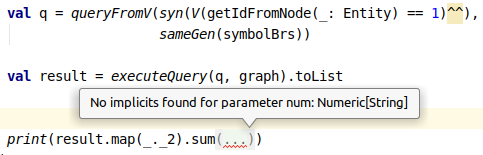
\includegraphics[width=0.48\textwidth]{pictures/image.png}

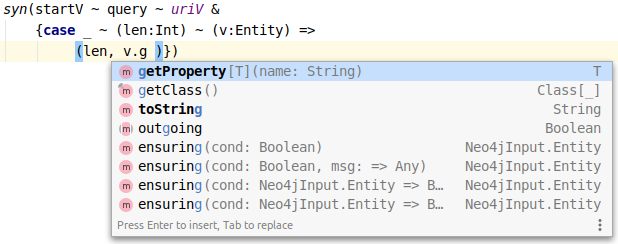
\includegraphics[width=0.48\textwidth]{pictures/image1.png}


Static type chacking

\subsection{User-Defined Actions}

We want to get all reachcbale vertices and collect inforamation about paths as a result of a query.
To do it we equip query with additional user-defined actions.

\subsection{IDE Support}

Screens!!!!
